\subsection{錐}
錐$\mathcal{K} \subseteq \mathbb{R}^n$とは任意の$\mathbf{x} \in \mathcal{K}, \alpha > 0$に対して、$\alpha \mathbf{x} \in \mathcal{K}$となるような集合のことをいい、集合$\mathcal{K}$が凸であるとは
\begin{align*}
  \mathbf{x}_1, \mathbf{x}_2 \in \mathcal{K}, \alpha_1, \alpha_2 \in \mathbb{R}
\end{align*}
に対して
\begin{align*}
  \alpha_1 + \alpha_2 = 1, \alpha_1, \alpha_2 \geq 0
\end{align*}
としたとき
\begin{align*}
  \alpha_1 \mathbf{x}_1 + \alpha_2 \mathbf{x}_2 \in \mathcal{K}
\end{align*}
となることをいう。凸な錐$\mathcal{K}$は凸錐と呼ばれ、その凸錐が閉集合の時、その錐のことを閉凸錐と呼ぶ。

$S_+^n$はこの定義のもと凸錐となる。実際、次の定理が成り立つ。
\begin{theorem}
  $S_+^n$は凸錐である。
\end{theorem}
\begin{proof}
  まず、$S_+^n$が錐であることを示す。$\alpha > 0$と任意のベクトル$\mathbf{x} \in \mathbb{R}^n$および$A \in S_+^n$に対して、$\alpha A$が$S_+^n$に入るかを確認する。そのために$\mathbf{x}^T \alpha A \mathbf{x}$が非負であるかを確かめる。まず、$\alpha$が非負の実数であることから
  \begin{align*}
    \mathbf{x}^T \alpha A \mathbf{x} = \alpha \mathbf{x}^T A \mathbf{x}
  \end{align*}
  となり、$A \in S_+^n$、$\alpha > 0$という仮定から$\mathbf{x}^T A \mathbf{x} \geq 0$より、$\alpha \mathbf{x}^T A \mathbf{x} \geq 0$。従って$\alpha A \in S_+^n$となるので$S_+^n$は錐である。

  次に、$S_+^n$が凸であることを示す。任意の$A, B \in S_+^n$、$\alpha, \beta \geq 0$に対して、$\alpha + \beta = 1$とする。任意のベクトル$\mathbf{x} \in \mathbf{R}^n$に対して、
  \begin{align*}
    \mathbf{x}^T \left(\alpha A + \beta B\right) \mathbf{x} = \alpha \mathbf{x}^T A \mathbf{x} + \beta \mathbf{x}^T B \mathbf{x}.
  \end{align*}
  ここで、仮定$A, B \in S_+^n$、つまり$\mathbf{x}^T A \mathbf{x} \geq 0, \mathbf{x}^T B \mathbf{x} \geq 0$および$\alpha, \beta \geq 0$から$\alpha \mathbf{x}^T A \mathbf{x} \geq 0$かつ$\beta \mathbf{x}^T B \mathbf{x} \geq 0$より、$\alpha \mathbf{x}^T A \mathbf{x} + \beta \mathbf{x}^T B \mathbf{x} \geq 0$。したがって、$\alpha \mathbf{x}^T A \mathbf{x} + \beta \mathbf{x}^T B \mathbf{x} \in S_+^n$。ゆえに$S_+^n$は凸である。

  以上から集合$S_+^n$は凸かつ錐となるので、$S_+^n$は凸錐である。
\end{proof}
\begin{figure}
  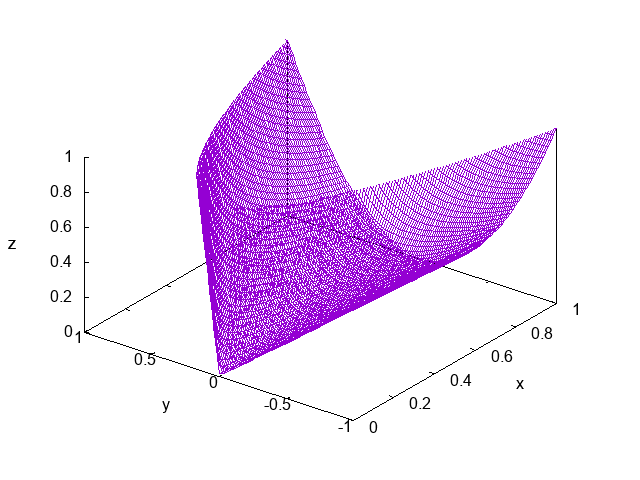
\includegraphics{PSDcone.png}
  \caption[]{$S_+^2$の図}
\end{figure}

\subsection{双対錐}
錐$\mathcal{K}$に対して
\begin{align*}
  \mathcal{K}^* = \Set{x | \forall y \in \mathcal{K}, \dot<x, y> \geq 0}
\end{align*}
を$\mathcal{K}$の双対錐という。特に双対錐が閉集合かつ凸であるとき、その双対錐のことを閉凸双対錐という。閉凸錐$\mathcal{K}$の双対錐$\mathcal{K}^*$の双対錐$\left(\mathcal{K}^*\right)^* = \mathcal{K}^{**}$は$\mathcal{K}$自身となる\cite*{ConvexOptimization}。

また、錐$\mathcal{K}$の双対錐$\mathcal{K}^*$が$\mathcal{K}$自身となるとき、すなわち
\begin{align*}
  \mathcal{K}^* = \mathcal{K}
\end{align*}
となる錐のことを自己双対錐という。このような錐の例としては$S_+^n$などがある。
